\documentclass[
  11pt,
  letterpaper,
   addpoints,
  answers
  ]{exam}

% Carga el preámbulo localizado en la carpeta superior
\NeedsTeXFormat{LaTeX2e}[2023/04/30]

% Provide the name of your page, the date it was last updated, and a comment about what it's used for
\ProvidesPackage{../exercise-preamble}[2023/04/30 Prof. Cassanelli custom LaTeX style]

% \usepackage{printlen}
% \uselengthunit{in}\printlength{\textwidth}

% PACKAGES
\usepackage[dvipsnames]{xcolor}

\usepackage{graphicx}
\graphicspath{{../figures}}
\usepackage{amsmath,amsthm,amssymb,mathtools,mathrsfs}
\usepackage{commath}
\usepackage{upgreek}
\usepackage{cancel}
\usepackage{enumerate}
\usepackage[font=small]{caption}
\usepackage[normalem]{ulem}
\usepackage{steinmetz}

\usepackage[left=1.5cm, right=1.5cm, top=1cm]{geometry}

% REFERENCES AND OTHERS
\usepackage{../aas_macros}
\usepackage{natbib}
\bibpunct{(}{)}{;}{a}{}{,}

\usepackage{tikz}
\usepackage{tikz-3dplot}
\usepackage{circuitikz}
\usepackage{pgfplots}
\pgfplotsset{compat=1.15}
\usepgfplotslibrary{smithchart}
\usetikzlibrary{
  decorations.pathmorphing,
  decorations.markings,
  calc,
  patterns,
  decorations,
  angles,
  quotes,
  ext.topaths.arcthrough,
  shapes
  }

\usepackage{siunitx}
\sisetup{
    range-phrase=\text{--},
    range-units=single,
    separate-uncertainty=true,
    print-unity-mantissa=false
    }
\DeclareSIUnit{\gauss}{G}
\DeclareSIUnit{\jansky}{Jy}

\newcommand{\iu}{\mathrm{i}\mkern1mu}
\newcommand{\ju}{\mathrm{j}\mkern1mu}
\newcommand{\euler}{\mathrm{e}}
\newcommand{\exponential}[1]{\mathrm{exp}\left[#1\right]}
\newcommand{\uvec}[1]{\widehat{\mathbf{#1}}}
\newcommand{\uvecs}[1]{\boldsymbol{\widehat{#1}}}
\newcommand{\bvec}[1]{\boldsymbol{\mathcal{#1}}}

\usepackage{hyperref}
\hypersetup{
    % bookmarks=true,
    unicode=true,
    pdftoolbar=true,
    pdfmenubar=true,
    pdffitwindow=false,
    pdfstartview={FitH},
    pdftitle={EL3103},
    pdfauthor={Tomas Cassanelli},
    pdfcreator={Tomas Cassanelli},
    pdfnewwindow=true,
    colorlinks=true,
    linkcolor=Violet,
    citecolor=Violet,
    urlcolor=Violet
    }

% Exam document class
\renewcommand{\figurename}{Figura}
\renewcommand{\tablename}{Cuadro}
\pagestyle{empty}

\usepackage[spanish]{cleveref}

\crefname{question}{\protect{pregunta}}{\protect{preguntas}}
\Crefname{question}{\protect{Pregunta}}{\protect{Preguntas}}
\creflabelformat{question}{#2{#1}#3}

\renewcommand{\solutiontitle}{\noindent\textbf{Solución:}\par\noindent}
\bracketedpoints
\pointname{~puntos}

\endinput

% Paquetes locales
\usepackage{float}
\usepackage{booktabs} % para \toprule, \midrule, \bottomrule
\usepackage{xcolor} % para colores
\usepackage{bm} % para negrita en símbolos matemáticos

% Macros locales
\newcommand{\Rel}{\mathfrak{R}} % símbolo para la reluctancia
\DeclareMathOperator{\Var}{Var} % operador de varianza

\begin{document}

% Configuración del encabezado usando comandos de la clase exam
\pagestyle{headandfoot}
\extraheadheight{0.5in} % Baja el encabezado aumentando el espacio superior
\firstpageheader{\textit{Análisis de Sistemas Dinámicos y Estimación}}{}{EL3204-1}
\runningheader{\textit{Análisis de Sistemas Dinámicos y Estimación}}{}{EL3204}
\firstpagefooter{}{\thepage}{}
\runningfooter{}{\thepage}{}
\headrule % Línea debajo del encabezado

% Numeración de página
\pagenumbering{arabic}

% Portada
\begin{center}
    \vspace*{1cm}
    
    % Logo superior
    \includegraphics[width=0.5\textwidth]{../fcfm_die}
    
    \vspace{2cm}
    
    % Líneas decorativas superiores
    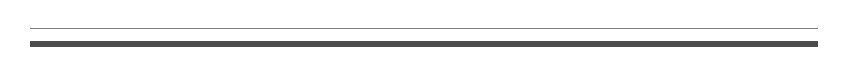
\begin{tikzpicture}
        \draw[line width=2pt, black!70] (0,0) -- (10,0);
        \draw[line width=0.5pt, black!50] (0,0.2) -- (10,0.2);
    \end{tikzpicture}
    
    \vspace{1cm}
    
    % Título principal
    {\fontsize{28}{34}\selectfont\bfseries 
    Análisis de Sistemas\\[0.3cm]
    Dinámicos y Estimación}
    
    \vspace{0.5cm}
    
    {\Large\textbf{EL3204-1}}
    
    \vspace{1cm}
    
    % Líneas decorativas inferiores
    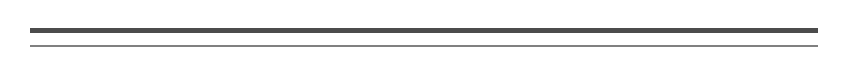
\begin{tikzpicture}
        \draw[line width=0.5pt, black!50] (0,0) -- (10,0);
        \draw[line width=2pt, black!70] (0,0.2) -- (10,0.2);
    \end{tikzpicture}
    
    \vspace{1.5cm}
    
    % Subtítulo
    {\LARGE\itshape Auxiliar 12 - Estimación}
    
    \vspace{0.5cm}
    {\large Prof Marcos Orchard - Sebastian Espinoza.}\\
    {\large Prof Auxiliar Erik Sáez Aravena.}
    
    % Decoración con símbolo matemático de fondo
    \begin{tikzpicture}[remember picture, overlay]
        \node[opacity=0.5, rotate=0] at ([yshift=-8cm]current page.center) {
            \fontsize{280}{300}\selectfont\color{black!15}$\mathcal{I}(\theta)$
        };
    \end{tikzpicture}
    
    \vfill
    
\end{center}

\newpage
%----------------------------
% =========================================
% Unidad III — Estimación de Parámetros (Resumen)
% =========================================
\section*{Resumen}

Este auxiliar cubre conceptos fundamentales de la teoría de estimación de parámetros, que complementa los temas de detección vistos anteriormente. En problemas de detección, el espacio paramétrico $\Theta$ era discreto y finito, pero ahora trabajamos con un conjunto \textbf{infinito no numerable} de posibles valores para el parámetro que queremos estimar (un continuo).

\subsection*{1. Conceptos Básicos de Estimación}
Algunos conceptos importante a considerar son:
\begin{enumerate}
\item \textbf{Espacio de observación ($\mathbb{X}$):} Espacio donde la variable aleatoria $X \in \mathbb{X}$ toma valores. Para vectores aleatorios, $\mathbb{X}^n$ representa el espacio producto.

  \item  \textbf{Espacio de decisión ($\Theta$):} En estimación, es un conjunto \textbf{infinito no numerable} de valores (a diferencia de detección donde era finito). Ejemplos: $\Theta = \mathbb{R}^+$ para estimar amplitudes, $\Theta = \mathbb{R}$ para estimar medias.

\item \textbf{Familia de distribuciones paramétricas ($J_\theta$):} Conjunto de distribuciones indexadas por $\theta$:
\[
J_\theta = \{P_X(x|\theta) : \theta \in \Theta\}
\]

\item \textbf{Estimador:} Una función $\hat{\theta}(x_1, \ldots, x_n)$ que depende de las observaciones y entrega una estimación del parámetro $\theta$ asociado a la distribución $P_X(x|\theta)$.
\end{enumerate}
\subsection*{2. Propiedades de los Estimadores}
\begin{enumerate}
  \item \textbf{Estimador Insesgado:} Un estimador $\hat{\theta}(x_1, \ldots, x_n)$ es insesgado si:
\[
\mathbb{E}[\hat{\theta}(X_1, \ldots, X_n)] = \theta
\]
Es decir, en promedio el estimador entrega el valor verdadero del parámetro.

\item \textbf{Estimador Asintóticamente Insesgado:} Si el sesgo tiende a cero cuando $n \to \infty$:
\[
\lim_{n\to\infty} \mathbb{E}[\hat{\theta}(X_1, \ldots, X_n)] = \theta
\]

\item \textbf{Estimador Consistente:} Un estimador es consistente si converge en probabilidad al valor verdadero:
\[
\lim_{n\to\infty} P_X(|\hat{\theta}(X_1, \ldots, X_n) - \theta| > \epsilon) = 0 \quad \forall \epsilon > 0
\]

\item \textbf{Observación:} Mediante la desigualdad de Chebyshev, si un estimador es insesgado y su varianza tiende a cero cuando $n \to \infty$, entonces es consistente:
\[
\lim_{n\to\infty} \Var(\hat{\theta}(X_1, \ldots, X_n)) = 0 \implies \text{consistencia}
\]
\end{enumerate}
\subsection*{3. Condiciones de Regularidad}

Las condiciones de regularidad permiten intercambiar el orden de derivación e integración en la función de verosimilitud. Bajo estas condiciones se cumple:
\begin{enumerate}
  \item \textbf{Primera condición:} La esperanza de la derivada de la log-verosimilitud es cero:
\[
\mathbb{E}_{X_1^n}\left[\frac{\partial \ln L(X_1, \ldots, X_n|\theta)}{\partial \theta}\right] = 0
\]

\item \textbf{Segunda condición:} La esperanza de un término específico es cero:
\[
\mathbb{E}_{X_1^n}\left[\frac{1}{L(X_1, \ldots, X_n|\theta)}\frac{\partial^2 L(X_1, \ldots, X_n|\theta)}{\partial \theta^2}\right] = 0
\]

\item \textbf{Identidad de Bartlett:} Relaciona la varianza con su segunda derivada:
\[
\mathbb{E}_{X_1^n}\left[\left(\frac{\partial \ln L}{\partial \theta}\right)^2\right] = -\mathbb{E}_{X_1^n}\left[\frac{\partial^2 \ln L}{\partial \theta^2}\right]
\]

Esta identidad permite calcular la información de Fisher de dos formas equivalentes.
\end{enumerate}
\subsection*{4. Información de Fisher}

La información de Fisher $\mathcal{I}(\theta)$ cuantifica cuánta información sobre el parámetro $\theta$ contienen las observaciones:
\[
\mathcal{I}(\theta) = \mathbb{E}\left[\left(\frac{\partial \ln f(X|\theta)}{\partial \theta}\right)^2\right] = -\mathbb{E}\left[\frac{\partial^2 \ln f(X|\theta)}{\partial \theta^2}\right]
\]

\textbf{Propiedad Aditiva:} Para muestras i.i.d., la información de Fisher es aditiva:
\[
\mathcal{I}_n(\theta) = n \cdot \mathcal{I}_1(\theta)
\]

Esta propiedad refleja que más observaciones independientes proporcionan más información sobre el parámetro.

\subsection*{5. Cota de Cramér-Rao}

La cota de Cramér-Rao establece un límite inferior para la varianza de cualquier estimador insesgado:
\[
\Var(\hat{\theta}) \geq \frac{1}{\mathcal{I}(\theta)}
\]
\begin{enumerate}
  \item \textbf{Estimador Eficiente:} Un estimador insesgado que alcanza la cota de Cramér-Rao se llama \textbf{eficiente} o \textbf{de mínima varianza}

\item \textbf{Interpretación:} La información de Fisher es inversamente proporcional a la mínima varianza posible. Más información $\implies$ menor varianza mínima.
\end{enumerate}
\subsection*{6. Estimador de Máxima Verosimilitud (ML)}

El estimador de máxima verosimilitud se obtiene maximizando la función de verosimilitud:
\[
\hat{\theta}_{ML} = \arg\max_{\theta} L(x_1, \ldots, x_n|\theta) = \arg\max_{\theta} \ln L(x_1, \ldots, x_n|\theta)
\]

\textbf{Propiedades del estimador ML:}
\begin{itemize}
    \item Bajo condiciones de regularidad, es asintóticamente insesgado
    \item Es consistente
    \item Es asintóticamente eficiente (alcanza la cota de Cramér-Rao cuando $n \to \infty$)
    \item Es invariante bajo transformaciones: si $\hat{\theta}_{ML}$ es el ML de $\theta$, entonces $g(\hat{\theta}_{ML})$ es el ML de $g(\theta)$
\end{itemize}

\textbf{Método de solución:} Criterio de la primera derivada:
\[
\frac{\partial \ln L(x_1, \ldots, x_n|\theta)}{\partial \theta}\bigg|_{\theta=\hat{\theta}_{ML}} = 0
\]

Verificar que la segunda derivada es negativa para confirmar que es un máximo.

\subsection*{7. Resumen de Verificaciones para un Estimador}

Para analizar completamente un estimador $\hat{\theta}$, verificar:

\begin{enumerate}
    \item \textbf{Insesgamiento:} Calcular $\mathbb{E}[\hat{\theta}]$ y verificar si es igual a $\theta$
    \item \textbf{Consistencia:} Verificar que $\lim_{n\to\infty} \Var(\hat{\theta}) = 0$ (si es insesgado)
    \item \textbf{Varianza:} Calcular $\Var(\hat{\theta})$ explícitamente
    \item \textbf{Eficiencia:} Calcular $\mathcal{I}(\theta)$ y comparar $\Var(\hat{\theta})$ con $\frac{1}{\mathcal{I}(\theta)}$
\end{enumerate}

%----------------------------
\newpage
\begin{questions}
\question
\label{q:estimador_exponencial}
Considere el problema de estimar $\theta \in \mathbb{R}$ dada una observación $X \in \mathbb{R}$, se sabe que la distribución condicional de $\Theta$ dado $X$ está dotada de la siguiente función de densidad condicional definida como:
\[
f_{\Theta|X}(\theta|x) = \begin{cases}
e^{-(\theta-x)}, & \text{si } \theta > x \\
0, & \text{si } x > \theta
\end{cases}
\]

Encuentre el estimador de mínimo error cuadrático medio y MAP.

\begin{solution}
Para este problema, tenemos la distribución a posteriori $f_{\Theta|X}(\theta|x)$ y debemos encontrar dos estimadores distintos.

\begin{itemize}
\item \textbf{Estimador de Mínimo Error Cuadrático Medio (MMSE):}

El estimador MMSE corresponde a la esperanza condicional:
\[
\hat{\theta}_{MMSE}(x) = \mathbb{E}[\Theta|X=x] = \int_{-\infty}^{\infty} \theta \cdot f_{\Theta|X}(\theta|x) d\theta
\]

Dada la función de densidad:
\[
f_{\Theta|X}(\theta|x) = \begin{cases}
e^{-(\theta-x)}, & \text{si } \theta > x \\
0, & \text{si } \theta \leq x
\end{cases}
\]
Entonces, la integral se reduce a:
\[
\hat{\theta}_{MMSE}(x) = \int_{x}^{\infty} \theta \cdot e^{-(\theta-x)} d\theta
\]

Realizamos el cambio de variable $u = \theta - x$, entonces:
\begin{itemize}
\item $\theta = u + x$
\item $d\theta = du$
\item Cuando $\theta = x$, tenemos $u = 0$
\item Cuando $\theta \to \infty$, tenemos $u \to \infty$
\end{itemize}

Sustituyendo en la integral:
\[
\hat{\theta}_{MMSE}(x) = \int_{0}^{\infty} (u + x) e^{-u} du
\]

Separamos la integral en dos términos:
\[
= \int_{0}^{\infty} u \cdot e^{-u} du + \int_{0}^{\infty} x \cdot e^{-u} du
\]

Como $x$ es una constante (no depende de $u$), podemos sacarlo de la integral:
\[
= \int_{0}^{\infty} u \cdot e^{-u} du + x \cdot \int_{0}^{\infty} e^{-u} du
\]

Ahora calculamos cada integral por separado:

\textbf{Primera integral:} $\int_{0}^{\infty} e^{-u} du$

Esta es una integral estándar de la exponencial:
\[
\int_{0}^{\infty} e^{-u} du = \left[-e^{-u}\right]_{0}^{\infty} = \lim_{u \to \infty}(-e^{-u}) - (-e^{0}) = 0 - (-1) = 1
\]

\textbf{Segunda integral:} $\int_{0}^{\infty} u \cdot e^{-u} du$

Usamos integración por partes. Recordemos que $\int v \, dw = vw - \int w \, dv$.

Elegimos:
\begin{itemize}
\item $v = u \implies dv = du$
\item $dw = e^{-u}du \implies w = -e^{-u}$
\end{itemize}

Aplicando la fórmula:
\[
\int_{0}^{\infty} u \cdot e^{-u} du = \left[u \cdot (-e^{-u})\right]_{0}^{\infty} - \int_{0}^{\infty} (-e^{-u}) du
\]

Simplificando:
\[
= \left[-u \cdot e^{-u}\right]_{0}^{\infty} + \int_{0}^{\infty} e^{-u} du
\]

Evaluamos el primer término:
\[
\left[-u \cdot e^{-u}\right]_{0}^{\infty} = \lim_{u \to \infty}\left(-u \cdot e^{-u}\right) - (0 \cdot e^{0}) = 0 - 0 = 0
\]

Nota: $\lim_{u \to \infty} u \cdot e^{-u} = 0$ porque la exponencial decrece más rápido que $u$ crece (aplicando L'Hôpital si es necesario).

El segundo término ya lo calculamos antes y vale $1$. Por lo tanto:
\[
\int_{0}^{\infty} u \cdot e^{-u} du = 0 + 1 = 1
\]

\textbf{Combinando ambas integrales:}
\[
\hat{\theta}_{MMSE}(x) = \int_{0}^{\infty} u \cdot e^{-u} du + x \cdot \int_{0}^{\infty} e^{-u} du = 1 + x \cdot 1 = x + 1
\]

Por lo tanto, el estimador MMSE es:
\[
\boxed{\hat{\theta}_{MMSE}(x) = x + 1}
\]

\item \textbf{Estimador MAP (Maximum A Posteriori)}:

El estimador MAP maximiza la densidad a posteriori:
\[
\hat{\theta}_{MAP}(x) = \arg\max_{\theta} f_{\Theta|X}(\theta|x)
\]

Recordemos que la función de densidad es:
\[
f_{\Theta|X}(\theta|x) = \begin{cases}
e^{-(\theta-x)}, & \text{si } \theta > x \\
0, & \text{si } \theta \leq x
\end{cases}
\]

Para encontrar el máximo, analizamos el comportamiento de $f_{\Theta|X}(\theta|x) = e^{-(\theta-x)}$ en la región donde $\theta > x$.

Calculamos la derivada con respecto a $\theta$:
\[
\frac{d}{d\theta} f_{\Theta|X}(\theta|x) = \frac{d}{d\theta} e^{-(\theta-x)} = -e^{-(\theta-x)}
\]

Como $e^{-(\theta-x)} > 0$ para todo $\theta$, tenemos que:
\[
\frac{d}{d\theta} f_{\Theta|X}(\theta|x) = -e^{-(\theta-x)} < 0 \quad \text{para todo } \theta > x
\]

La derivada es siempre negativa en la región donde la función está definida, lo que significa que $f_{\Theta|X}(\theta|x)$ es una función estrictamente decreciente.

Por lo tanto, el máximo de $f_{\Theta|X}(\theta|x)$ se alcanza en el valor más pequeño posible de $\theta$, que es $\theta = x$ (el límite inferior de la región donde la función es no nula).

Evaluando en ese punto:
\[
f_{\Theta|X}(x|x) = e^{-(x-x)} = e^0 = 1
\]

Y para cualquier $\theta > x$:
\[
f_{\Theta|X}(\theta|x) = e^{-(\theta-x)} < 1
\]

Concluimos que el estimador MAP es:
\[
\boxed{\hat{\theta}_{MAP}(x) = x}
\]

\vspace{0.5cm}

\textbf{Interpretación:}
\begin{itemize}
\item El estimador MAP $\hat{\theta}_{MAP}(x) = x$ elige el valor que maximiza la probabilidad a posteriori.
\item El estimador MMSE $\hat{\theta}_{MMSE}(x) = x + 1$ considera toda la distribución a posteriori y minimiza el error cuadrático medio esperado, resultando en un valor desplazado una unidad respecto al MAP debido a la forma asimétrica de la distribución exponencial.
\end{itemize}
\end{itemize}
\end{solution}

\question
\label{q:estimador_normal_bayesiano}
Sean $X_1, \ldots, X_n$ muestras i.i.d. de la variable aleatoria $X \sim \mathcal{N}(\mu, \sigma^2)$. A su vez, $\mu$ es una variable aleatoria continua tal que $\mu \sim \mathcal{N}(0, \sigma_0^2)$.

\begin{enumerate}
\item Determine las densidades $f_{X_1, \ldots, X_n}(x_1, \ldots, x_n|\theta)$ y $f_{\mu}$.
\item Obtenga el estimador MAP de $\mu$, $\hat{\mu}_{MAP}$.
\item Determine los casos límite en que $\sigma_0^2 \longrightarrow \infty$ y $\sigma_0^2 \longrightarrow 0$. Interprete cada situación.
\end{enumerate}

\begin{solution}

\textbf{1. Determine las densidades $f_{X_1, \ldots, X_n}(x_1, \ldots, x_n|\theta)$ y $f_{\mu}$.}

Como se ha visto en auxiliares anteriores, se tiene la siguiente densidad conjunta condicional para el vector $X$:
\[
f_X(x_1, \ldots, x_n|\mu) = \prod_{i=1}^{n} f_{X_i}(x|\mu) = \prod_{i=1}^{n} \frac{1}{\sqrt{2\pi\sigma^2}} \cdot e^{-\frac{(x_i-\mu)^2}{2\sigma^2}}
\]

\[
f_X(x_1, \ldots, x_n|\mu) = \left(\frac{1}{2\pi\sigma^2}\right)^{\frac{n}{2}} \cdot e^{-\frac{1}{2\sigma^2}\sum_{i=1}^{n}(x_i-\mu)^2}
\]

Por otro lado, la densidad de $\mu$ es una normal conocida:
\[
f_{\mu}(\mu) = \frac{1}{\sqrt{2\pi\sigma_0^2}} \cdot e^{-\frac{\mu^2}{2\sigma_0^2}}
\]

\textbf{2. Obtenga el estimador MAP de $\mu$, $\hat{\mu}_{MAP}$.}

Por definición, se tiene que el estimador MAP es:
\[
\hat{\mu}_{MAP} = \arg\max_{\mu} \ln[f_X(x_1, \ldots, x_n|\mu) \cdot f_{\mu}(\mu)]
\]

Obtengamos la expresión a maximizar:
\begin{align*}
\ln[f_X(x_1, \ldots, x_n|\mu) \cdot f_{\mu}(\mu)] &= -\frac{n}{2}\ln(2\pi\sigma^2) - \frac{1}{2\sigma^2} \cdot \sum_{i=1}^{n}(x_i - \mu)^2 - \frac{1}{2}\ln(2\pi\sigma_0^2) - \frac{\mu^2}{2\sigma_0^2}
\end{align*}

Luego, aplicamos el criterio de la primera derivada:
\begin{align*}
\frac{d}{d\mu}\left(-\frac{n}{2}\ln(2\pi\sigma^2) - \frac{1}{2\sigma^2} \cdot \sum_{i=1}^{n}(x_i - \mu)^2 - \frac{1}{2}\ln(2\pi\sigma_0^2) - \frac{\mu^2}{2\sigma_0^2}\right) &= 0 \\
\frac{1}{\sigma^2} \cdot \sum_{i=1}^{n}(x_i - \mu) - \frac{\mu}{\sigma_0^2} &= 0 \\
\frac{1}{\sigma^2}\sum_{i=1}^{n}x_i - \frac{n\mu}{\sigma^2} - \frac{\mu}{\sigma_0^2} &= 0 \\
\frac{\sum_{i=1}^{n}x_i}{\sigma^2} &= \mu \cdot \left(\frac{1}{\sigma_0^2} + \frac{n}{\sigma^2}\right) \\
\mu &= \frac{\sum_{i=1}^{n}x_i}{\sigma^2 \cdot \left(\frac{1}{\sigma_0^2} + \frac{n}{\sigma^2}\right)} \\
\mu &= \frac{\sum_{i=1}^{n}x_i}{\left(\frac{\sigma^2}{\sigma_0^2} + n\right)} \\
\Longleftrightarrow \mu &= \frac{\sigma_0^2}{n\sigma_0^2 + \sigma^2} \cdot \sum_{i=1}^{n}x_i \\
\Longrightarrow \mu &= \frac{\sigma_0^2}{\sigma_0^2 + \frac{\sigma^2}{n}} \cdot \frac{1}{n} \cdot \sum_{i=1}^{n}x_i
\end{align*}

Luego, el estimador MAP de $\mu$ corresponde a:
\[
\boxed{\hat{\mu}_{MAP} = \frac{\sigma_0^2}{\sigma_0^2 + \frac{\sigma^2}{n}} \cdot \frac{1}{n} \cdot \sum_{i=1}^{n}x_i}
\]

\textbf{3. Determine los casos límite en que $\sigma_0^2 \longrightarrow \infty$ y $\sigma_0^2 \longrightarrow 0$. Interprete cada situación.}

Nos pondremos en ambos casos:

\begin{itemize}
\item $\sigma_0^2 \longrightarrow \infty$: En este caso tenemos que ver el límite del estimador:
\[
\lim_{\sigma_0^2 \to \infty} \frac{\sigma_0^2}{\sigma_0^2 + \frac{\sigma^2}{n}} \cdot \frac{1}{n} \cdot \sum_{i=1}^{n}x_i = \frac{1}{n} \cdot \sum_{i=1}^{n}x_i
\]

Podemos notar de este caso que, mientras más incerteza tenemos sobre el parámetro $\mu$ en su distribución (equivalente a que la varianza de la normal sea muy grande), el estimador MAP tiende a la media empírica de las observaciones, es decir, los datos son los que determinan el estimador (Porque le creemos más a los datos que al conocimiento a priori). A su vez corresponde al estimador de máxima verosimilitud del problema.

\item $\sigma_0^2 \longrightarrow 0$: En este caso tenemos que ver el límite del estimador:
\[
\lim_{\sigma_0^2 \to 0} \frac{\sigma_0^2}{\sigma_0^2 + \frac{\sigma^2}{n}} \cdot \frac{1}{n} \cdot \sum_{i=1}^{n}x_i = \frac{1}{\sigma^2} \cdot \sum_{i=1}^{n}x_i
\]

En este caso ocurre que tenemos mucha certeza sobre el valor del estimador lo cual se modela como $\sigma_0^2 \longrightarrow 0$. Esto genera que el estimador MAP quede dependa solo del número de observaciones y de la varianza de las observaciones. Esto se traduce a que se tiene con tanta certeza el valor del estimador MAP, que si $\sigma_0^2 \to 0$ entonces su valor siempre será su esperanza, en este caso 0. El estimador MAP sí entrega un valor aproximado pero como se tiene certeza total no es necesario.
\end{itemize}
\end{solution}

\question
\label{q:particulas_radiactivas}
Considere que tiene un cuerpo radiactivo el cual, dentro de un cierto intervalo de tiempo, emite $\Theta$ partículas. Sin embargo, usted mide cada una de estas emisiones con un detector imperfecto, el cual tiene probabilidad $p$ de detectar correctamente cada partícula.

Si $B_i^\Theta$ son las variables aleatorias que indican si cada partícula es detectada correctamente o no, de modo que $B_i \sim \text{Bernoulli}(p)$, entonces la variable de medición $X$ corresponde a
\[
X = \sum_{i=1}^{\Theta} B_i,
\]
correspondiente al total de partículas que fueron correctamente detectadas.

Gracias a estudios previos, usted sabe que $\Theta \sim \text{Poisson}(\lambda)$, con $\lambda$ una propiedad del cuerpo radiactivo. Con esto, determine el estimador de mínimo error cuadrático medio (MMSE) para estimar el número de partículas a partir de las mediciones.

\begin{solution}
Sabemos que el estimador MMSE $\hat{\theta}_{MMSE}(x)$ está dado por
\[
\hat{\theta}_{MMSE}(x) = \mathbb{E}\{\Theta|X = x\},
\]
por lo que para encontrarlo necesitamos expresar la distribución a posteriori. Para esto, notemos que por Bayes
\[
P_{\Theta|X}(\theta|x) = \frac{P_{X|\Theta}(x|\theta)P_{\Theta}(\theta)}{P_X(x)},
\]
donde
\[
P_{X|\Theta}(x|\theta) = \binom{\theta}{x}p^x(1-p)^{\theta-x}, \quad P_{\Theta}(\theta) = \frac{e^{-\lambda}\lambda^{\theta}}{\theta!}.
\]

Para el término del denominador, aplicamos la \textbf{ley de probabilidades totales}, que nos dice que para calcular la probabilidad marginal de $X$ debemos sumar sobre todos los posibles valores de $\Theta$:
\[
P_X(x) = \sum_{\theta \in \mathbb{N}} P_{X|\Theta}(x|\theta)P_{\Theta}(\theta) = \sum_{\theta \geq 0} P_{X|\Theta}(x|\theta)P_{\Theta}(\theta)
\]

Ahora bien, recordemos que $X|\Theta$ sigue una distribución binomial: $X|\Theta=\theta \sim \text{Binomial}(\theta, p)$, donde $X$ representa el número de éxitos (partículas detectadas) en $\theta$ intentos. Por la naturaleza de la binomial, es imposible obtener más éxitos que intentos, es decir, $X \leq \Theta$. Esto significa que:
\[
P_{X|\Theta}(x|\theta) = \binom{\theta}{x}p^x(1-p)^{\theta-x} = 0 \quad \text{si } \theta < x
\]

porque el coeficiente binomial $\binom{\theta}{x} = \frac{\theta!}{x!(\theta-x)!}$ no está definido (o es cero) cuando $\theta < x$ (ya que $(\theta-x)!$ sería el factorial de un número negativo, que no existe). Por lo tanto, todos los términos con $\theta < x$ no contribuyen a la suma, y podemos escribir:
\begin{align*}
P_X(x) &= \sum_{\theta \geq 0} P_{X|\Theta}(x|\theta)P_{\Theta}(\theta) \\
&= \sum_{\theta \geq x} P_{X|\Theta}(x|\theta)P_{\Theta}(\theta) \\
&= \sum_{\theta \geq x} \binom{\theta}{x}p^x(1-p)^{\theta-x}\frac{e^{-\lambda}\lambda^{\theta}}{\theta!} \\
&= \sum_{\theta \geq x} \frac{\theta!}{x!(\theta-x)!}p^x(1-p)^{\theta-x}\frac{e^{-\lambda}\lambda^{\theta}}{\theta!} \\
&= \sum_{\theta \geq x} \frac{1}{x!(\theta-x)!}p^x(1-p)^{\theta-x}e^{-\lambda}\lambda^{\theta} \\
&= \frac{e^{-\lambda}p^x}{x!} \sum_{\theta \geq x} \frac{1}{(\theta-x)!}(1-p)^{\theta-x}\lambda^{\theta} \\
&= \frac{e^{-\lambda}(\lambda p)^x}{x!} \sum_{\theta \geq x} \frac{(\lambda(1-p))^{\theta-x}}{(\theta-x)!},
\end{align*}
donde, considerando el cambio de variable $i = \theta - x$, podemos ver que la serie corresponde a $e^{\lambda(1-p)} = e^{\lambda}e^{-\lambda p}$, por lo que tenemos
\[
P_X(x) = \frac{e^{-\lambda p}(\lambda p)^x}{x!},
\]
indicando que $X \sim \text{Poisson}(\lambda p)$. Reemplazando, vemos que la distribución a posteriori (limitándose al rango $\theta \geq x$) corresponde a
\begin{align*}
P_{\Theta|X}(\theta|x) &= \frac{P_{X|\Theta}(x|\theta)P_{\Theta}(\theta)}{P_X(x)} \\
&= \frac{\frac{\theta!}{x!(\theta-x)!}p^x(1-p)^{\theta-x}\frac{e^{-\lambda}\lambda^{\theta}}{\theta!}}{\frac{e^{-\lambda p}(\lambda p)^x}{x!}} \\
&= \frac{e^{-\lambda(1-p)}(\lambda(1-p))^{\theta-x}}{(\theta-x)!},
\end{align*}
correspondiente a una Poisson desplazada. Luego, calculando la esperanza tenemos
\begin{align*}
\hat{\theta}_{MMSE}(x) &= \mathbb{E}\{\Theta|X = x\} \\
&= \sum_{\theta \geq x} \theta P_{\Theta|X}(\theta|x) \\
&= \sum_{\theta \geq x} \theta \frac{e^{-\lambda(1-p)}(\lambda(1-p))^{\theta-x}}{(\theta-x)!} \qquad / \; i = \theta - x \\
&= e^{-\lambda(1-p)} \sum_{i \geq 0} (i+x) \frac{(\lambda(1-p))^i}{i!} \\
&= e^{-\lambda(1-p)} \left[\sum_{i \geq 0} i \frac{(\lambda(1-p))^i}{i!} + x \sum_{i \geq 0} \frac{(\lambda(1-p))^i}{i!}\right].
\end{align*}

\textbf{Cálculo del primer término:} Para la suma $\sum_{i \geq 0} i \frac{(\lambda(1-p))^i}{i!}$, notamos que el término con $i=0$ es cero, por lo que podemos escribir:
\begin{align*}
\sum_{i \geq 0} i \frac{(\lambda(1-p))^i}{i!} &= \sum_{i \geq 1} i \frac{(\lambda(1-p))^i}{i!} \\
&= \sum_{i \geq 1} i \frac{(\lambda(1-p))^i}{i \cdot (i-1)!} \quad \text{(usando que $i! = i \cdot (i-1)!$)} \\
&= \sum_{i \geq 1} \frac{(\lambda(1-p))^i}{(i-1)!}.
\end{align*}

Ahora, realizamos el cambio de variable $j = i - 1$, lo cual implica que $i = j + 1$. Cuando $i = 1$, tenemos $j = 0$, y cuando $i \to \infty$, tenemos $j \to \infty$. Además, $(\lambda(1-p))^i = (\lambda(1-p))^{j+1} = \lambda(1-p) \cdot (\lambda(1-p))^j$. Por lo tanto:
\begin{align*}
\sum_{i \geq 1} \frac{(\lambda(1-p))^i}{(i-1)!} &= \sum_{j \geq 0} \frac{(\lambda(1-p))^{j+1}}{j!} \\
&= \lambda(1-p) \sum_{j \geq 0} \frac{(\lambda(1-p))^{j}}{j!} \\
&= \lambda(1-p) \cdot e^{\lambda(1-p)}.
\end{align*}

\textbf{Cálculo del segundo término:} Para la suma $\sum_{i \geq 0} \frac{(\lambda(1-p))^i}{i!}$, reconocemos la serie de Taylor de la exponencial:
\[
\sum_{i \geq 0} \frac{(\lambda(1-p))^i}{i!} = e^{\lambda(1-p)}.
\]

\textbf{Combinando ambos términos:} Reemplazando en la expresión original:
\begin{align*}
\hat{\theta}_{MMSE}(x) &= e^{-\lambda(1-p)} \left[\lambda(1-p) \cdot e^{\lambda(1-p)} + x \cdot e^{\lambda(1-p)}\right] \\
&= e^{-\lambda(1-p)} \cdot e^{\lambda(1-p)} \left[\lambda(1-p) + x\right] \\
&= \lambda(1-p) + x \\
&= x + \lambda(1-p),
\end{align*}
de modo que el estimador MMSE está dado por
\[
\boxed{\hat{\theta}_{MMSE}(x) = x + \lambda(1-p).}
\]

Podemos ver que, pese a que $\Theta \in \mathcal{A} = \mathbb{N}$ (es decir, el problema es de detección), dado que $\lambda \in \mathbb{R}^+$ y $p \in (0,1)$ el estimador elige valores dentro de $\mathbb{R}^+$, y por lo tanto el problema se trata, indirectamente, como uno de estimación.
\end{solution}
\end{questions}
\end{document}